\section{Methodology} \label{sec:methodology_preliminary_results}

%\textcolor{blue}{
%Methodology:
%\begin{itemize}
%    \item Research Design:
%    \item Data Collection: Hierarchical datasets (e.g., sales data, economic indicators).
%    \item Methods: Implementing hierarchical models, applying XAI techniques, analyzing feature importance and reasoning.
%    \item Evaluation: Accuracy metrics and interpretability assessment.
%\end{itemize}
%}

Our preliminary research focusses on the methodological aspects of applying feature importance techniques to hierarchical forecasting models.
This includes adaptation of existing methods, but also tool development to support the analysis of hierarchical forecasting models.
Later we plan to conduct an empirical study to evaluate the methods on real-world datasets.

Our initial research design\ref{fig:research_design} includes the following steps:
\begin{itemize}
    \item Data collection: identify datasets with hierarchical time series data describing sales/demand for multiple product categories and regions with exogenous variables.
    \item Tool evaluation: assess the applicability of existing libraries for hierarchical forecasting and XAI techniques.
    \item Model implementation: we build global models that consider multiple series and exogenous variables.
    \item Feature importance analysis: We apply model attribution methods and aggregation and decomposition techniques to identify key features and analyze their impact on the forecast.
    \item Model reasoning: analyze the feature contributions to forecast and identify underlying rules on different levels of the hierarchy.
\end{itemize}


\begin{figure}
    \centering
\begin{tikzpicture}[node distance=2cm]

%\node (start) [startstop] {Start};
\node (data) [process] {Data Collection};
\node (tool) [process, below of=data] {Tool Evaluation};
\node (model) [process, below of=tool] {Model Implementation};
\node (importance) [process, below of=model] {Feature Importance Analysis};
\node (reasoning) [process, below of=importance] {Model Reasoning};
%\node (stop) [startstop, below of=reasoning] {End};

%\draw [arrow] (start) -- (data);
\draw [->] (data) -- (tool);
\draw [->] (tool) -- (model);
\draw [->] (model) -- (importance);
\draw [->] (importance) -- (reasoning);
%\draw [arrow] (reasoning) -- (stop);

% Annotations
%\node [annotation, right=3cm of data.east, anchor=west] (dataann) {
%    \begin{itemize}
%        \item Find hierarchical time series data.
%        \item Include sales/demand across categories and regions.
%        \item Add relevant exogenous variables.
%    \end{itemize}
%};
%
%\node [annotation, right=3cm of model.east, anchor=west] (modelann) {
%    \begin{itemize}
%        \item Build global models for multiple time series.
%        \item Integrate exogenous variables.
%    \end{itemize}
%};
%
%\node [annotation, right=3cm of importance.east, anchor=west] (importanceann) {
%    \begin{itemize}
%        \item Determine feature importance.
%        \item Use aggregation and decomposition.
%        \item Assess feature impact on forecasts.
%    \end{itemize}
%};
%
%\node [annotation, right=3cm of reasoning.east, anchor=west] (reasoningann) {
%    \begin{itemize}
%        \item Analyze feature contributions.
%        \item Discover rules at different hierarchy levels.
%    \end{itemize}
%};
\end{tikzpicture}
\caption{Research design} \label{fig:research_design}
\end{figure}





%The research design includes the following steps:
%\begin{itemize}
%    \item Data collection: we will use datasets with hierarchical time series data describing sales/demand for multiple product categories and regions.
%    \item Model implementation: we build global models that consider multiple series and exogenous variables. The ML models include decision trees, random forests, and gradient boosting.
%    \item Feature importance analysis: we apply model attribution methods such as PFIs, SHAP and SAGE to identify key features and analyze their impact on the forecast.
%    \item Model reasoning: analyze the feature contributions to forecast and identify the underlying rules.
%\end{itemize}

\subsection{Data collection and preprocessing}\label{subsec:data-collection-and-preprocessing}
%
%To model the hierarchical impact of features on forecasting, we must use datasets with multiple series and exogenous variables that represent demand drivers.
%There are multiple open sales data sets available; however, there are just a few, such as the M5 competition\citep{makridakis_m5_2022} and the Kaggle datasets\cite{favorita-sales}.
%For our initial exploration, we sampled M5 competition\citep{makridakis_m5_2022} dataset, which includes sales data for multiple product categories and regions.
%The dataset contains daily sales information for 3049 products in 10 stores over 5 years.
%For our analysis, we identified three products that have similar sales patterns and are sold in two states and five stores.
%As products are from the same category and department, the hierarchy at the product level was not considered.
%The reason for this filtering is to reduce the complexity of the model and to focus on the feature importance analysis.
%The selected products are FOODS\_3\_586, FOODS\_3\_080, and FOODS\_3\_555 and are sold in three states of Texas (TX), Wisconsin (WI).
%The total sales data for these products are shown in Figure \ref{fig:product_sales}.
%Our hierarchical structure is shown in Figure \ref{fig:hierarchical_structure}.
%It should be mentioned that the hierarchical structure can be inverted, meaning that the products can be at the top level and the stores at the bottom level,
%so technically our data set is grouped time series data.

\begin{figure}
    \centering
    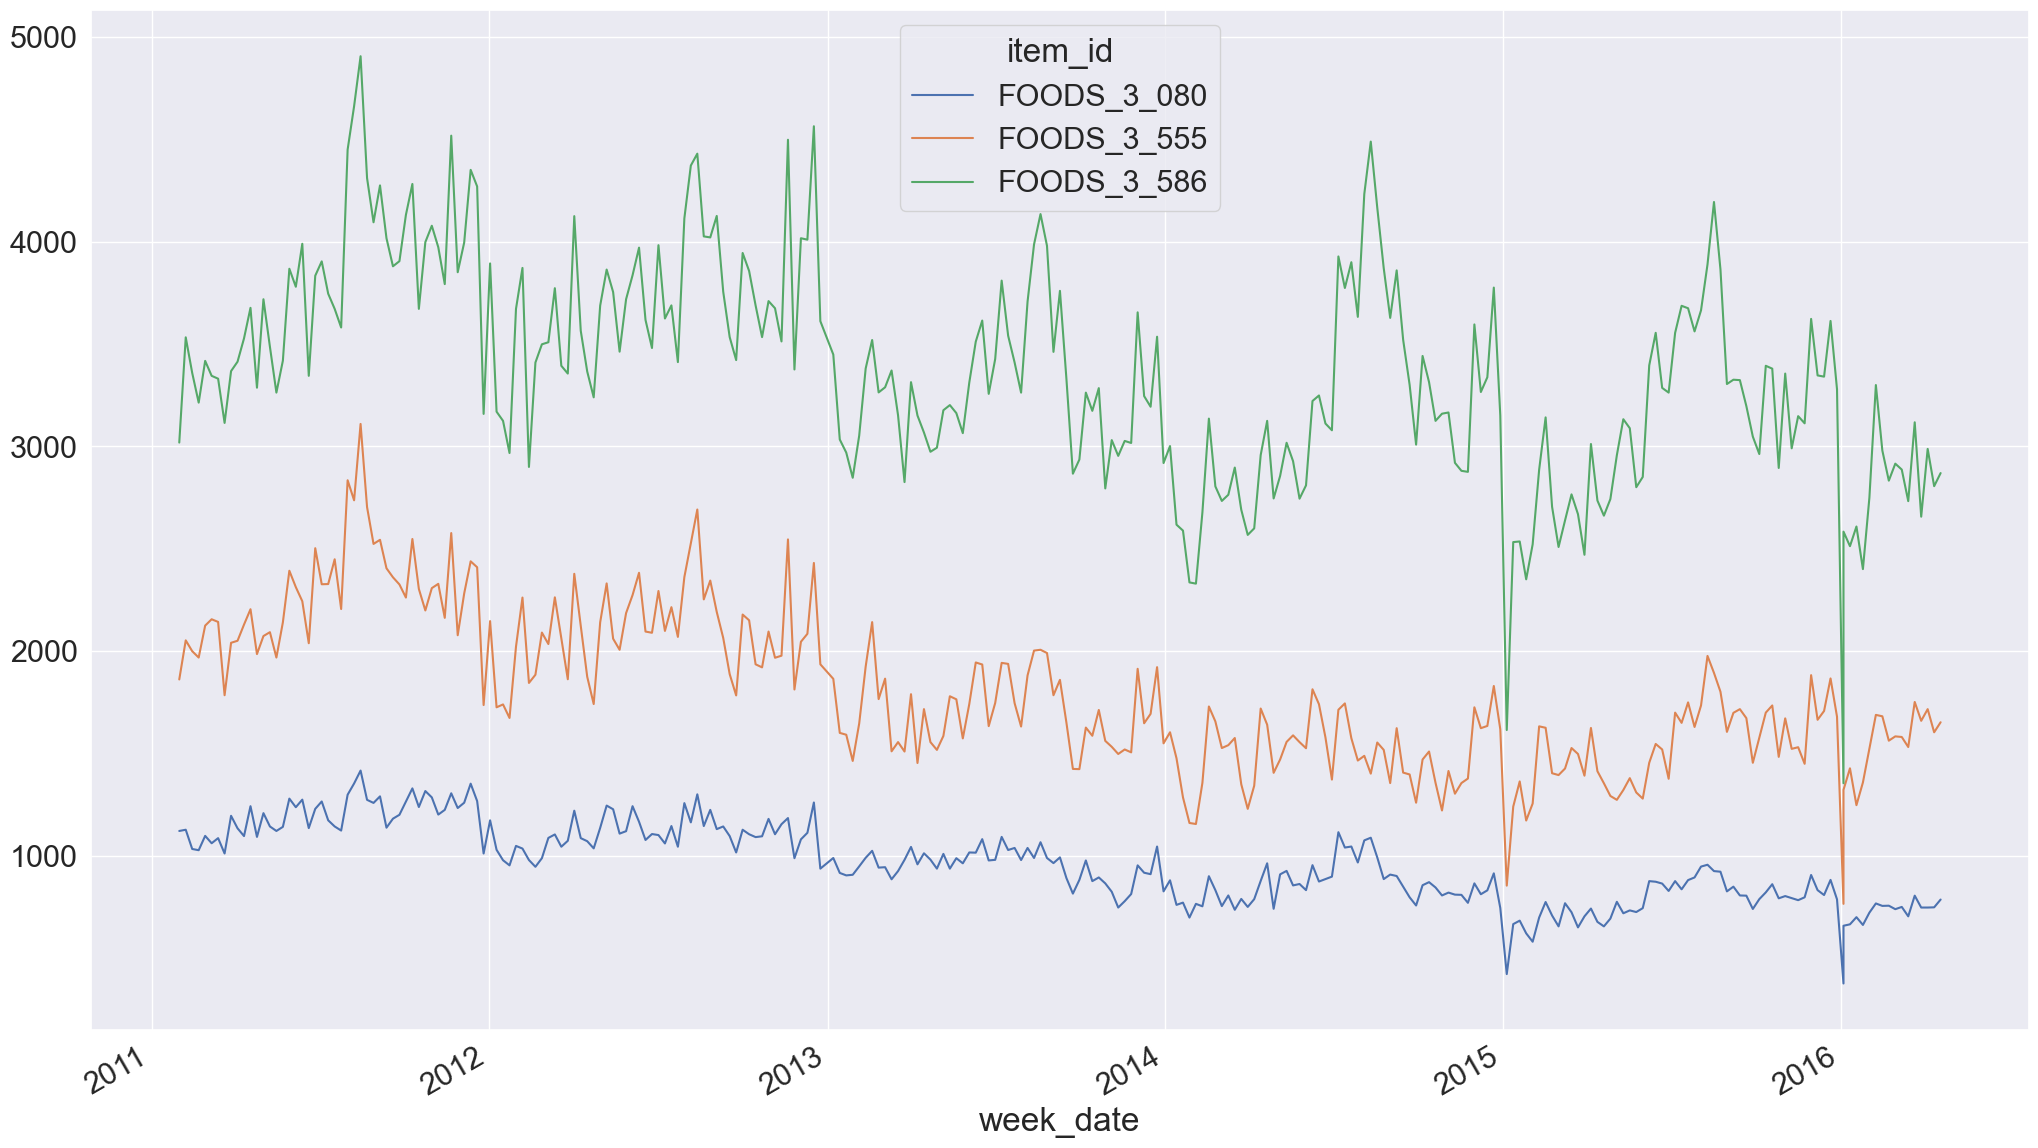
\includegraphics[width=0.8\linewidth]{sections/img/product_sales}
    \centering
    \caption{Total weekly sales for the chosen products}
    \label{fig:product_sales}
\end{figure}


%The sales we aggregated the data at the weekly level.
%\begin{itemize}
%    \item Aggregating data at the weekly level.
%    \item Splitting data into training and test sets.
%\end{itemize}


\begin{figure}
    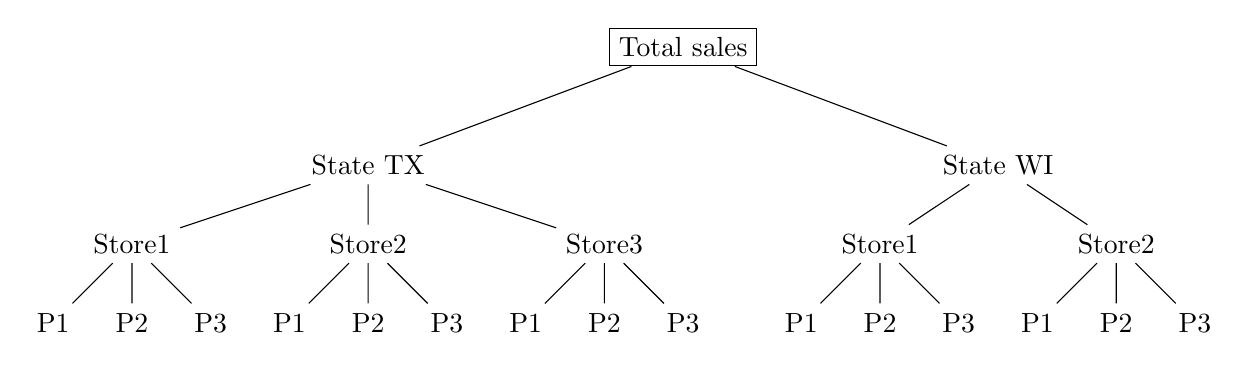
\begin{tikzpicture}
    [level 1/.style={sibling distance=80mm, level distance=15mm},
        level 2/.style={sibling distance=30mm, level distance=10mm},
        level 3/.style={sibling distance=10mm, level distance=10mm}]
        \node[rectangle,draw] {Total sales}
        child {node {State TX}
        child {node {Store1}
        child {node {P1}}
        child {node {P2}}
        child {node {P3}}
        }
        child {node {Store2}
        child {node {P1}}
        child {node {P2}}
        child {node {P3}}
        }
        child {node {Store3}
        child {node {P1}}
        child {node {P2}}
        child {node {P3}}
        }
        }
        child {node {State WI}
        child {node {Store1}
        child {node {P1}}
        child {node {P2}}
        child {node {P3}}
        }
        child {node {Store2}
        child {node {P1}}
        child {node {P2}}
        child {node {P3}}
        }
        };
    \end{tikzpicture}
    \caption{Hierarchical structure of product sales data (P1-3 = Product1-3)} \label{fig:hierarchical_structure}
\end{figure}

Data preprocessing two main parts: preparing the sales data and the exogenous variables.
Sales data were aggregated at the weekly level.
The weeks at the beginning and end of the data set were removed to have a consistent time period.
As features, lagged sales data was included to capture the temporal dependencies.
The exogenous variables were related to pricing and calendar events.
The selling price was already aggregated at the weekly level for each store and product.
Calendar events included whether a day was a holiday, had special events, and if it was a SNAP (Supplemental Nutrition Assistance Programme) day in a respective state.
To include these variables in some way, they were counted for each week and state.
In addition, the week of the year was included as a feature to capture seasonality.
The data were split into training and test sets, and the last complete year(2015) was used to test the model.
The structure of the data sales data is shown in Table \ref{tab:data_structure} and the exogenous variables in Table \ref{tab:exog_data_structure}.


%\end{table}

\begin{table}
    \centering
    \begin{resizebox}{\linewidth}{!}

        \begin{tabular}{
            |p{0.15\textwidth} % feature name
            |p{0.1\textwidth}  % feature type
            |p{0.75\textwidth}  % feature description
            |}
            \hline
            Feature name  & Type   & Description                                                                                         \\
            \hline
            week\_date    & date   & Starting date of week used for aggregation                                                          \\
            \hline
            week          & int    & Week number of the year                                                                             \\
            \hline
            series\_id    & string & Unique identifier for the series made of state+store+product combination,  representing the hierarchy \\
            \hline
            sales         & float  & Total sales for the week                                                                            \\
            \hline
            lag\_\emph{n} & float  & Sales from the previous \emph{n} weeks                                                              \\
            \hline
        \end{tabular}%
    \end{resizebox}
    \caption{ Sales data structure}
    \label{tab:data_structure}
\end{table}


\begin{table}
    \begin{tabular}{
        |p{0.15\textwidth} % feature name
        |p{0.1\textwidth}  % feature type
        |p{0.75\textwidth}  % feature description
        |}
        \hline
        Feature name    & Type   & Description                                                                                          \\
        \hline
        week\_date      & date   & Starting date of week used for aggregation                                                           \\
        \hline
        week\_of\_year  & int    & Week number of the year                                                                              \\
        \hline
        series\_id      & string & Unique identifier for the series made of state+store+product combination, representing the hierarchy \\
        \hline
        sell\_price     & float  & Selling price for the week for                                                                       \\
        \hline
        num\_of\_events & int    & The number of special events and holidays in the week                                                \\
        \hline
        snap\_days      & int    & Number of SNAP days in the week                                                                      \\
        \hline
    \end{tabular}
    \caption{Exogenous variables}
    \label{tab:exog_data_structure}
\end{table}

%\subsection{Model implementation}\label{subsec:model-implementation}
%The modelling approach is to build a single global on all series and exogenous variables for bottom-up aggregation.
%For creating forecast models, the skforecast\cite{skforecast} library was used.
%The base model for hierarchical forecasting was LightGBM~\cite{guolin_ke_highly_2017}
% due to its efficiency and also because of its widespread usage in the M5 competition in this data set\cite{makridakis_m5_2022}.
%Other ensemble models such as Random Forest or Gradient Boosting Machines could be used as well.
%Other reasons for choosing LightGBM are that it can handle categorical variables without the need for one-hot encoding, and that it supports model-specific split and gain-based global feature importance methods.
%
%Hyperparameter tuning was performed using the Optuna library\cite{optuna_2019}, by Bayesian optimisation.
%The search space\ref{tab:hyperparam_search_space} was defined for the parameters of the LightGBM model, including the number of predictors, the minimum number of samples in the leaf, and the maximum depth of the tree.
%In addition, the number of lagged sales records used as features was included in the search space.
%For the search, the data was split into training and validation sets, the last year being the validation set used for backtesting.
%The performance of the model was evaluated as a mean square error (MSE) in the validation set for each configuration.
%The best configuration found was with 239 estimators and a maximum depth of 26 with a backtesting MSE 4263.01
%The lagged sales records used as features were 1, 4, 5, 13, and 52 weeks.
%\begin{table}
%    \centering
%    \begin{tabular}{|l|l|l|}
%        \hline
%        Parameter          & Search space & Description                                             \\
%        \hline
%        n\_estimators      & 50-1000      & Number of boosting iterations                           \\
%        max\_depth         & 5-50         & Maximum depth of the tree                               \\
%        min\_samples\_leaf & 1-10         & Minimum number of samples required to be at a leaf node \\
%        num\_lagged\_sales & 4-52         & Number of lagged sales records used as features         \\
%        \hline
%    \end{tabular}
%    \caption{Model hyperparameters search space}
%    \label{tab:hyperparam_search_space}
%\end{table}
%
%The feature input for the final model is a table with the following columns:
%\begin{itemize}
%    \item week\_of\_year represented as numerical values (1-52)
%    \item sell\_price for the week for the product in the store
%    \item num\_of\_events for the week
%    \item snap\_days for the week in the state
%    \item lag\_\emph{n} for n in [1, 4, 5, 13, 52] representing the sales from the previous weeks
%    \item series\_id noted as (\_level\_skforecast) encoded as a numerical value representing the series hierarchy
%\end{itemize}
%\emph{Series\_id} could have been encoded as a one-hot encoded vector or as a categorical variable given it is supported by LightGBM.
%One-hot encoded vector would have increased the number of features and the complexity of the model,
%while with the categorical variable


% Lags: [ 1  4  5 13 52]
%  Parameters: {'n_estimators': 239, 'max_depth': 26}
%%Backtesting metric: 4263.010292888604

%\subsection{Feature importance analysis and model reasoning}\label{subsec:feature-importance-analysis-and-model-reasoning}
%Two initial ideas were considered to analyse the importance of characteristics.
%The first involves using the mean SHAP values for cohorts representing different levels of the hierarchy, providing information on the contribution of features throughout the structure.
%The second approach is based on conditional permutation importance, which evaluates the importance of features while
%accounting for the hierarchical structure on the idea of subgroup-based permutation importance\cite{cond_pfi}.
%The first method was prioritised for implementation due to the availability of support in the SHAP library\cite{scott_lundberg_consistent_2018}.
%Given an instance $x$ for prediction, the SHAP value of the feature $i$ is $\phi_i(x)$
%Each $x$ is part of a cohort $C_k$ based on the series hierarchy $k$.
%The contribution value or importance of feature $i$ for a $C_{k}$ cohort is calculated as
%\begin{equation}
%    \phi_i(C_k) = \frac{1}{|C_k|} \sum_{x \in C_k} |{\phi_i(x)|}
%\end{equation}
%where $|C_k|$ is the cardinality of $C_k$ and $|{\phi_i(x)}|$ is the absolute SHAP value of feature, $i$ for instance $x$.
%%$\bar{\phi}_i(C)$.
%
%Steps for the feature importance analysis:
%\begin{itemize}
%    \item For each prediction instance $x$ and feature \(i\) calculate SHAP value $\phi_i(x)$.
%    \item Split the instances into cohorts according to the hierarchy levels.
%    \item Calculate the mean SHAP values for each cohort $C$
%    \item Visualize the mean SHAP values for $C$ and summary plots
%\end{itemize}
%
%The reasoning of the model is based on the analysis of the contributions of the features to the forecast.
%The aim is to identify the underlying rules and patterns that the model uses to make predictions.
%The SHAP values provide a way to understand the impact of the features on the forecast.
%The analysis can be done at different levels of the hierarchy, from the global model to the state and store levels.


%\textcolor{red}{TODO: finish the description of the feature importance analysis}

%\subsection{SHAP values for hierarchical models} \label{subsec:shap_values}
%Methodology:
%
%Our goal is to evaluate the applicability of feature importance techniques to global(multi-series and multivariate) hierarhical
%models and analyze differences.
%Our planned methodology includes the following steps:
%\begin{itemize}
%    \item Data collection: we will use datasets with hierarchical time series data describing sales/demand for multiple product categories and regions.
%    \item Model implementation: we build global models that consider multiple series and exogenous variables. The ML models include decision trees, random forests, and gradient boosting.
%    \item Feature importance analysis: we apply model attribution methods such as PFIs, SHAP and SAGE to identify key features and analyze their impact on the forecast.
%    \item Model reasoning: analyze the feature contributions to forecast and identify the underlying rules.
%\end{itemize}


%\begin{itemize}
%    \item Initial findings on feature importance and model reasoning using XAI techniques for hierarchical models.
%    \item Observations on model performance and key features at different levels.
%\end{itemize}


\section{Preliminary Results}\label{sec:preliminary_results}

The preliminary results focus mainly on the practical application of SHAP values in hierarchical forecasting models
rather than on the theoretical aspects of feature importance.
As preliminary results, we present mean average SHAP values at different aggregation levels.
These provide an overview of the main contributors to the forecast at different levels of the hierarchy.

Furthermore, we visualise the distribution of SHAP values at different aggregation levels using violin plots,
which provide a representation of variability and density of SHAP values for each feature across the hierarchy.
This double representation allows for a more detailed analysis of the contribution of features to the forecast, for example,
if a feature contributes positively or negatively to the forecast.
In the following, we present several cases of different aggregation levels, starting from the global level to the store and product level,
but it is not meant to be exhaustive.

%\subsection{Global SHAP values} \label{subsec:global_shap}

At the global level, the SHAP values\ref{fig:global_shap} show that the most important features are the lagged sales values, especially the sales value of lag 1, which has the highest SHAP value.
This is expected as prior sales are the most important factor in predicting future sales.
The violin plot in Figure \ref{fig:global_shap_violin} shows the distribution of SHAP values for each feature.
It shows that the actual impact of the lag value is most of the time negative,
as after a week with higher sales, demand the following week can drop.

\begin{figure}[h]
    \centering
    \begin{minipage}{.45\textwidth}
        \centering
        \begin{subfigure}{\textwidth}
            \centering
            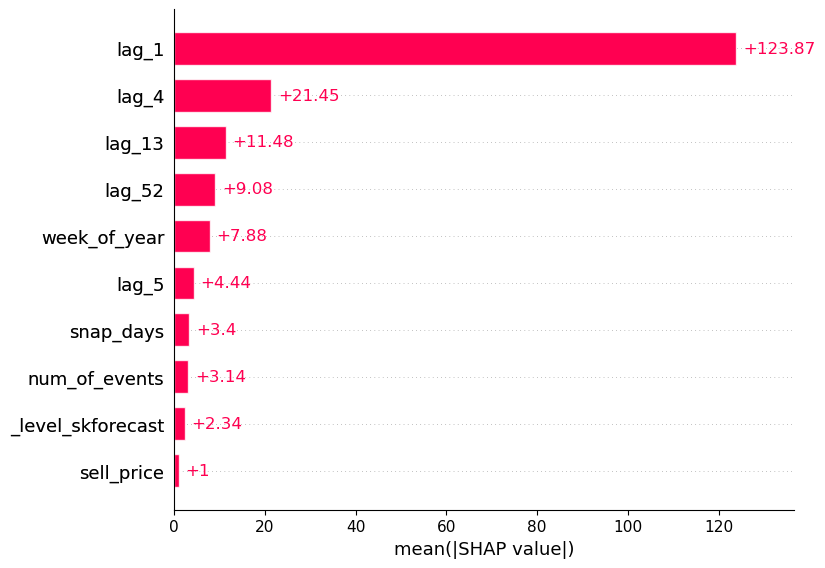
\includegraphics[width=\linewidth]{sections/img/shap_global}
            \caption{Global SHAP values}
            \label{fig:global_shap}
        \end{subfigure}%
%        \vskip\baselineskip
        \begin{subfigure}{\textwidth}
            \centering
            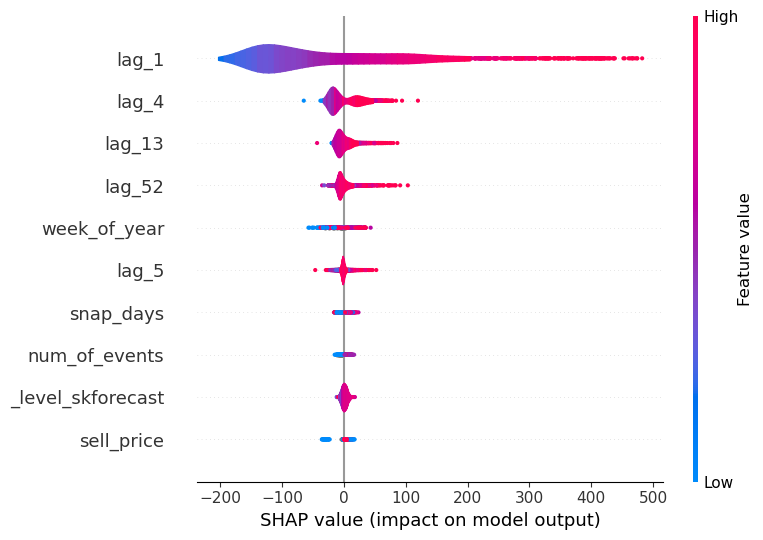
\includegraphics[width=\linewidth]{sections/img/shap_global_vioalin}
            \caption{Global SHAP violin plot}
            \label{fig:global_shap_violin}
        \end{subfigure}%
    \end{minipage}%
    \hfill
    \begin{minipage}{.45\textwidth}
        \centering
        % Add any additional subfigures here if needed
    \end{minipage}
    \caption{Global summary}\label{fig:global_summary}
\end{figure}


%%%%%%%%%%%%%%%%%%%%%%%%%%%%%%%%

%\subsection{State level SHAP values} \label{subsec:state_shap}
In case of state-level grouping, the number of samples differs for the two groups,
one of them having only two stores included.
This can be observed in the wider distribution on the violin plot of the Texas(TX) state.

\begin{figure}
    \centering
    \begin{minipage}{.45\textwidth}
        \centering
        \begin{subfigure}{\textwidth}
            \centering
            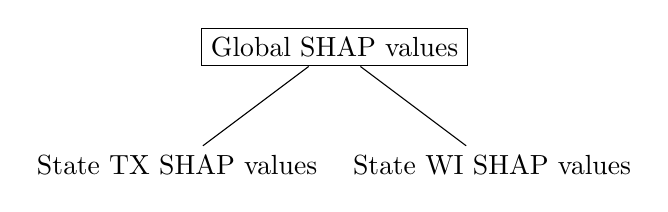
\begin{tikzpicture}
            [level 1/.style={sibling distance=40mm},
                level 2/.style={sibling distance=15mm}]
                \node[rectangle,draw] {Global SHAP values}
                child {node {State TX SHAP values} }
                child {node {State WI SHAP values}};
            \end{tikzpicture}
            \caption{State level SHAP values}
        \end{subfigure}%
        \vskip\baselineskip
        \begin{subfigure}{\textwidth}
            \centering
            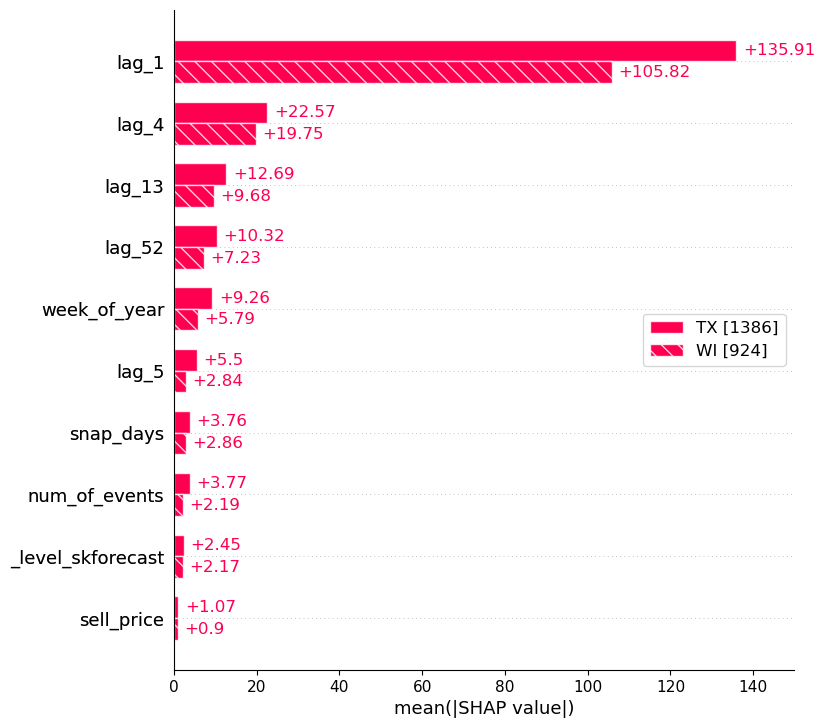
\includegraphics[width=\linewidth]{sections/img/state_product}
            \caption{State level SHAP values}
            \label{fig:sub2}
        \end{subfigure}%
    \end{minipage}%
    \hfill
    \begin{minipage}{.45\textwidth}
        \centering
        \begin{subfigure}{\textwidth}
            \centering
            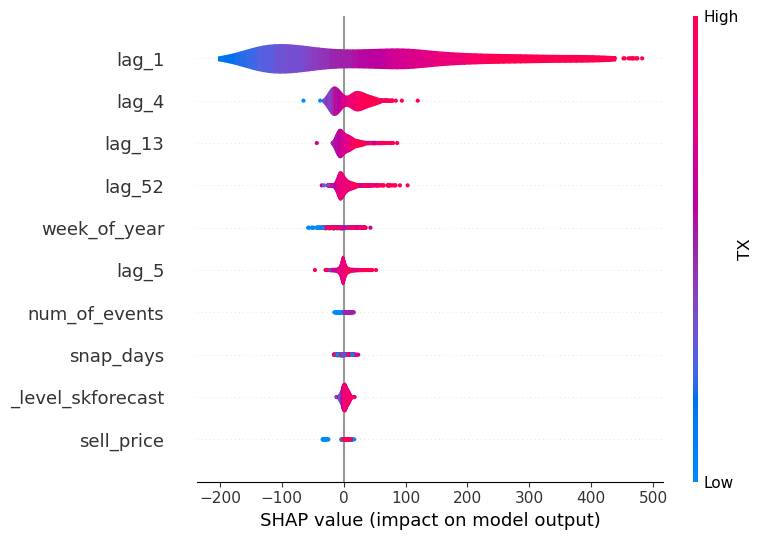
\includegraphics[width=\linewidth]{sections/img/state_tx_violin}
            \caption{TX state product SHAP summary}
            \label{fig:state_tx_violin_sub3}
        \end{subfigure}%
        \vskip\baselineskip
        \begin{subfigure}{\textwidth}
            \centering
            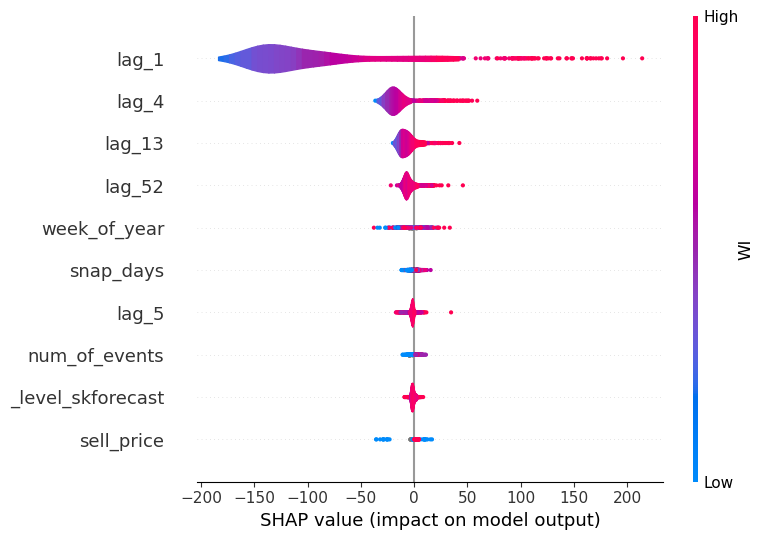
\includegraphics[width=\linewidth]{sections/img/state_wi_violin}
            \caption{WI state product SHAP summary}
            \label{fig:State_wi_violin_sub4}
        \end{subfigure}
    \end{minipage}
\end{figure}
%############################################################

%\subsection{State and product grouping}\label{subsec:state_prod_shap}
% TODO: The first lag value almost every time positively affects the forecast
\begin{figure}
    \centering
    \begin{minipage}{.45\textwidth}
        \centering
        \begin{subfigure}{\textwidth}
            \centering
            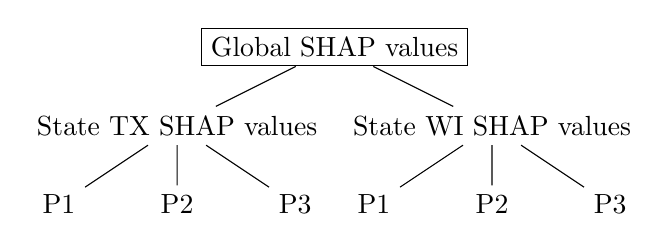
\begin{tikzpicture}
            [level 1/.style={sibling distance=40mm, level distance=10mm},
                level 2/.style={sibling distance=15mm, level distance=10mm}]
                \node[rectangle,draw] {Global SHAP values}
                child {node {State TX SHAP values}
                child {node {P1}}
                child {node {P2}}
                child {node {P3}}
                }
                child {node {State WI SHAP values}
                child {node {P1}}
                child {node {P2}}
                child {node {P3}}
                };
            \end{tikzpicture}
            \caption{Aggregation levels}
        \end{subfigure}%
        \vskip\baselineskip
        \begin{subfigure}{\textwidth}
            \centering
            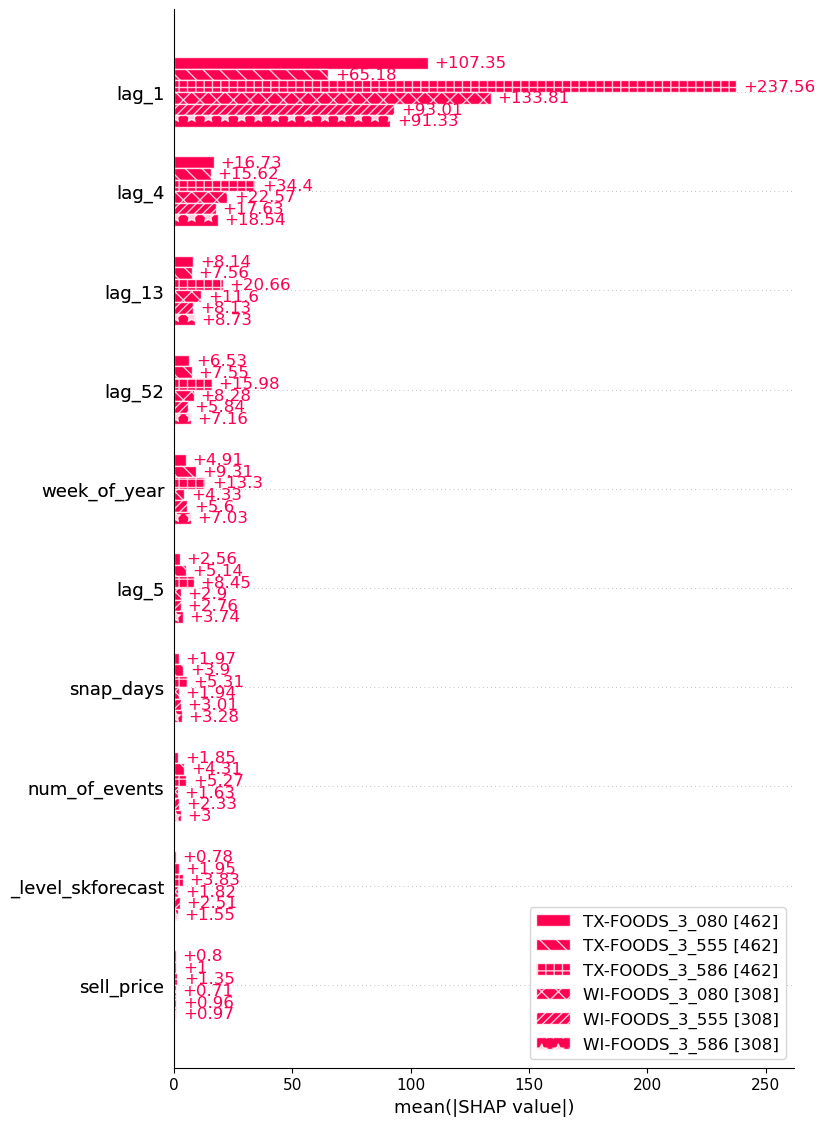
\includegraphics[width=\linewidth]{sections/img/bar_state_product}
            \caption{State and product level SHAP values}
            \label{fig:state_product_sub2}
        \end{subfigure}%
    \end{minipage}%
    \hfill
    \begin{minipage}{.45\textwidth}
        \centering
        \begin{subfigure}{\textwidth}
            \centering
            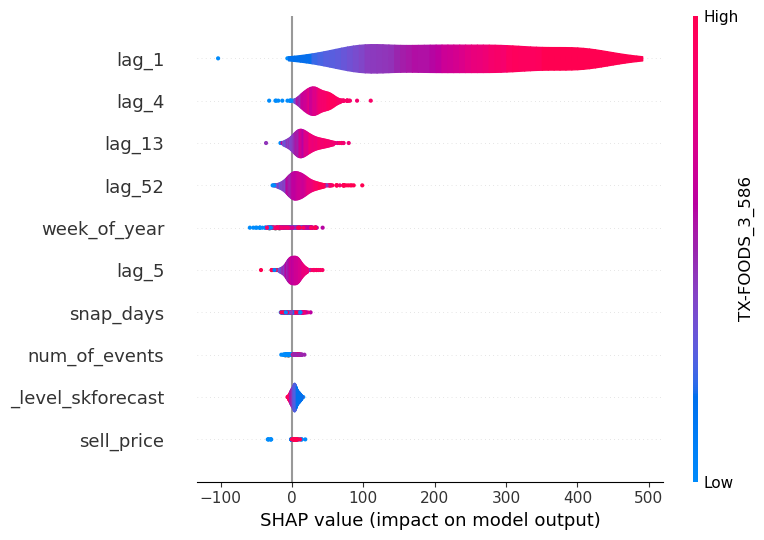
\includegraphics[width=\linewidth]{sections/img/state_product_violin_1}
            \caption{TX state FOODS\_3\_586 product SHAP summary}
            \label{fig:state_prod_sub3}
        \end{subfigure}%
        \vskip\baselineskip
        \begin{subfigure}{\textwidth}
            \centering
            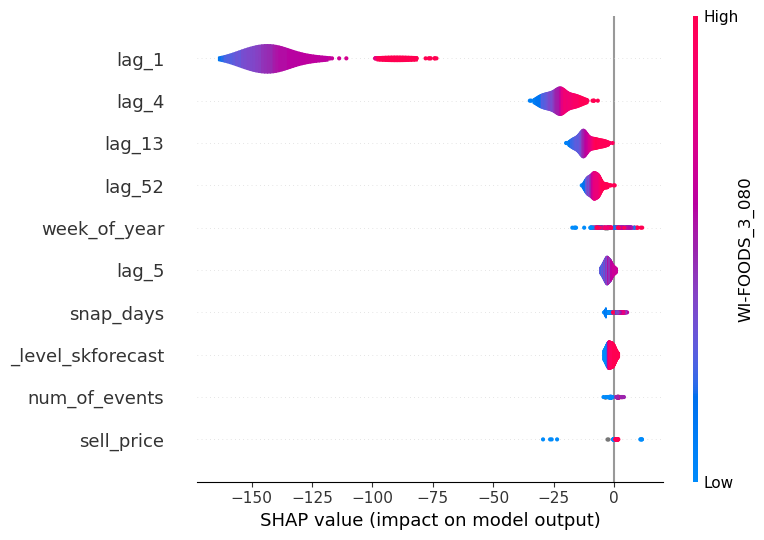
\includegraphics[width=\linewidth]{sections/img/state_product_violin2}
            \caption{WI state FOODS\_3\_080 product SHAP summary}
            \label{fig:state_prod_violin_sub4}
        \end{subfigure}
    \end{minipage}
    \caption{State and product level summary}
\end{figure}
%\begin{figure}
%    \centering
%%    \begin{tabular}{ c c }
%    \begin{subfigure}{.5\textwidth}
%        \centering
%        \begin{tikzpicture}
%        [level 1/.style={sibling distance=40mm, level distance=10mm},
%            level 2/.style={sibling distance=15mm, level distance=10mm}]
%            \node[rectangle,draw] {Global SHAP values}
%            child {node {State TX SHAP values}
%            child {node {P1}}
%            child {node {P2}}
%            child {node {P3}}
%            }
%            child {node {State WI SHAP values}
%            child {node {P1}}
%            child {node {P2}}
%            child {node {P3}}
%            };
%        \end{tikzpicture}
%        \caption{Aggregation levels}
%    \end{subfigure}%
%%    \vskip   \baselineskip
%    \begin{subfigure}{.5\textwidth}
%        \centering
%        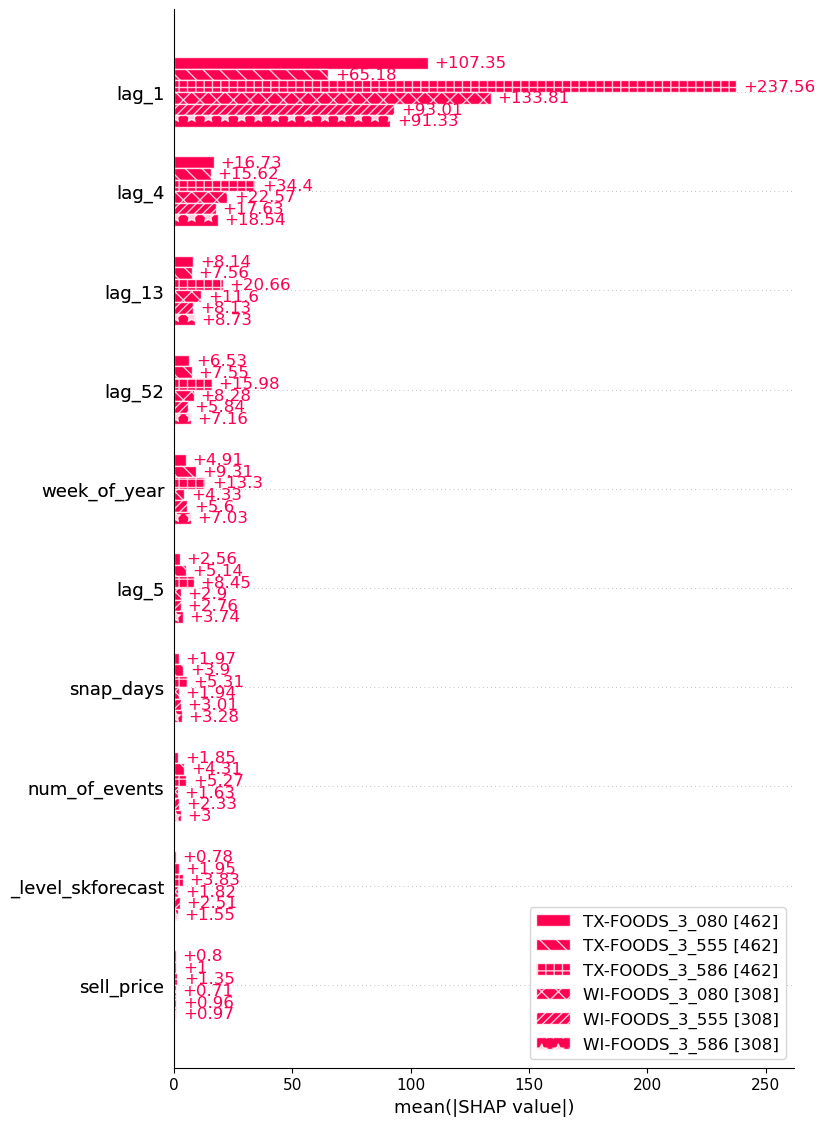
\includegraphics[width=\linewidth]{sections/img/bar_state_product}
%        \caption{State and product level SHAP values}
%        \label{fig:state_product_sub2}
%    \end{subfigure}%
%    \hskip  % \baselineskip
%    \begin{subfigure}{.5\textwidth}
%        \centering
%        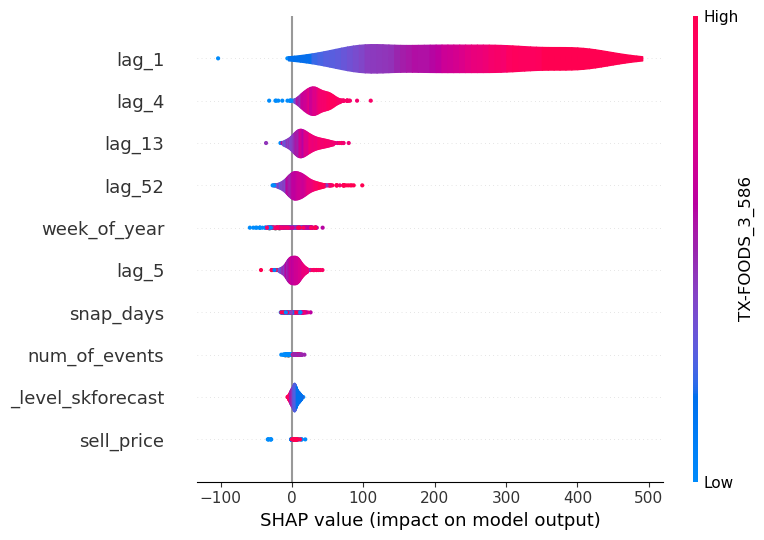
\includegraphics[width=\linewidth]{sections/img/state_product_violin_1}
%        \caption{TX state FOODS\_3\_586 product SHAP summary}
%        \label{fig:state_prod_sub3}
%    \end{subfigure}  %
%    \begin{subfigure}{.5\textwidth}
%        \centering
%        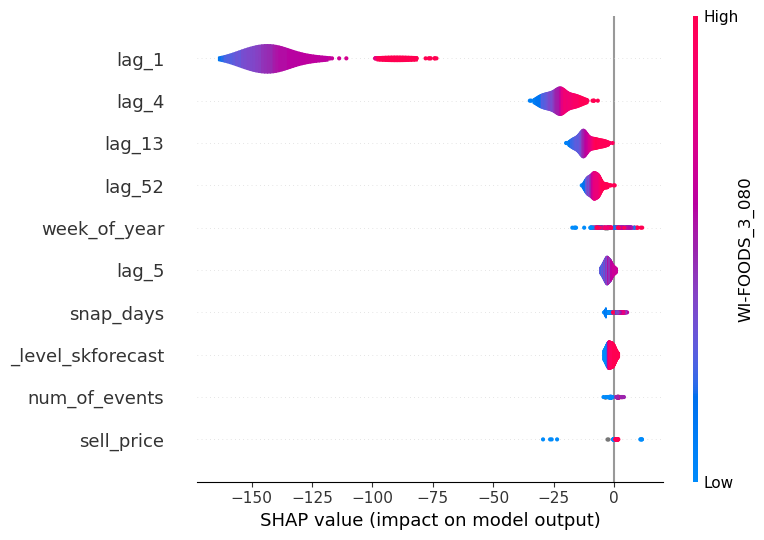
\includegraphics[width=\linewidth]{sections/img/state_product_violin2}
%        \caption{WI state FOODS\_3\_080 product SHAP summary}
%        \label{fig:state_prod_violin_sub4}
%    \end{subfigure}
%    \caption{State and product level summary}
%%    \end{tabular}
%\end{figure}



%%%%%%%%%%%%%%%%%%%%%%%%%%%%%%%%%%%%%%%%%%%%%%%%%%%%%%%%%%%%

% Store and product level
On the lowest level of the hierarchy presented in Figure \ref{fig:store_product_summary},
deviations can be revealed in the order of importance of the features.
For example, in Figure \ref{fig:store_prod_violin_sub4e} the week-of-year feature has a greater impact
on the forecast than some of the lag values that occurred in other cases in Figure \ref{fig:store_prod_sub3}.
This can be due to the fact that the store TX\_2 has a different seasonality pattern or
might have recurring special events, since the number of events is also a feature with higher impact on this store.
What is problematic in this case is that, due to the large number of series,
representation of the mean absolute SHAP value is hardly comprehensible in the previous form of the bar plot.
As a workaround, the grouping of feature contribution of each group is presented in Figure \ref{fig:store_product_sub2}.
What can be misleading in this case is the lack of order by impact and a different scale of the $x$ axis for each feature.

\begin{figure}
    \centering
    \begin{subfigure}{\textwidth}
        \centering
        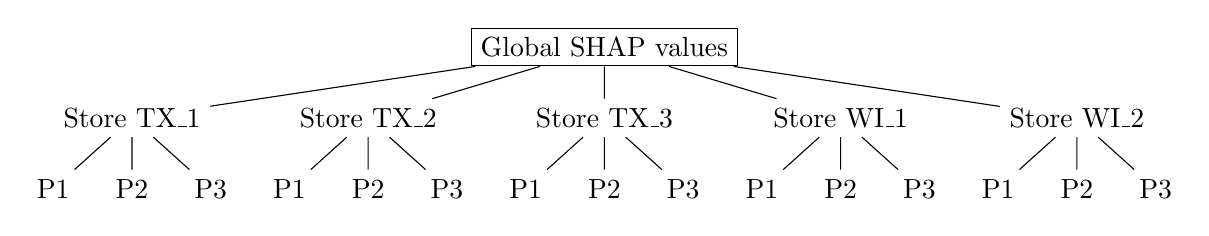
\begin{tikzpicture}
        [level 1/.style={sibling distance=30mm, level distance=9mm},
            level 2/.style={sibling distance=10mm,  level distance=9mm},]
%            level 3/.style={sibling distance=10mm}]
            \node[rectangle,draw] {Global SHAP values}
%            child {node {State TX}
            child {node {Store TX\_1}
            child {node {P1}}
            child {node {P2}}
            child {node {P3}}
            }
            child {node {Store TX\_2}
            child {node {P1}}
            child {node {P2}}
            child {node {P3}}
            }
            child {node {Store TX\_3}
            child {node {P1}}
            child {node {P2}}
            child {node {P3}}
            }
%            }
%            child {node {State WI}
            child {node {Store WI\_1}
            child {node {P1}}
            child {node {P2}}
            child {node {P3}}
            }
            child {node {Store WI\_2}
            child {node {P1}}
            child {node {P2}}
            child {node {P3}}
            };
        \end{tikzpicture}
        \caption{Aggregation levels}
    \end{subfigure}%
    \vskip\baselineskip
    \begin{subfigure}{.9\linewidth}
        \centering
     %  \includegraphics[width=0.8\linewidth, trim={0 67cm 30cm 0},clip ]{sections/img/store_product_shap2}
      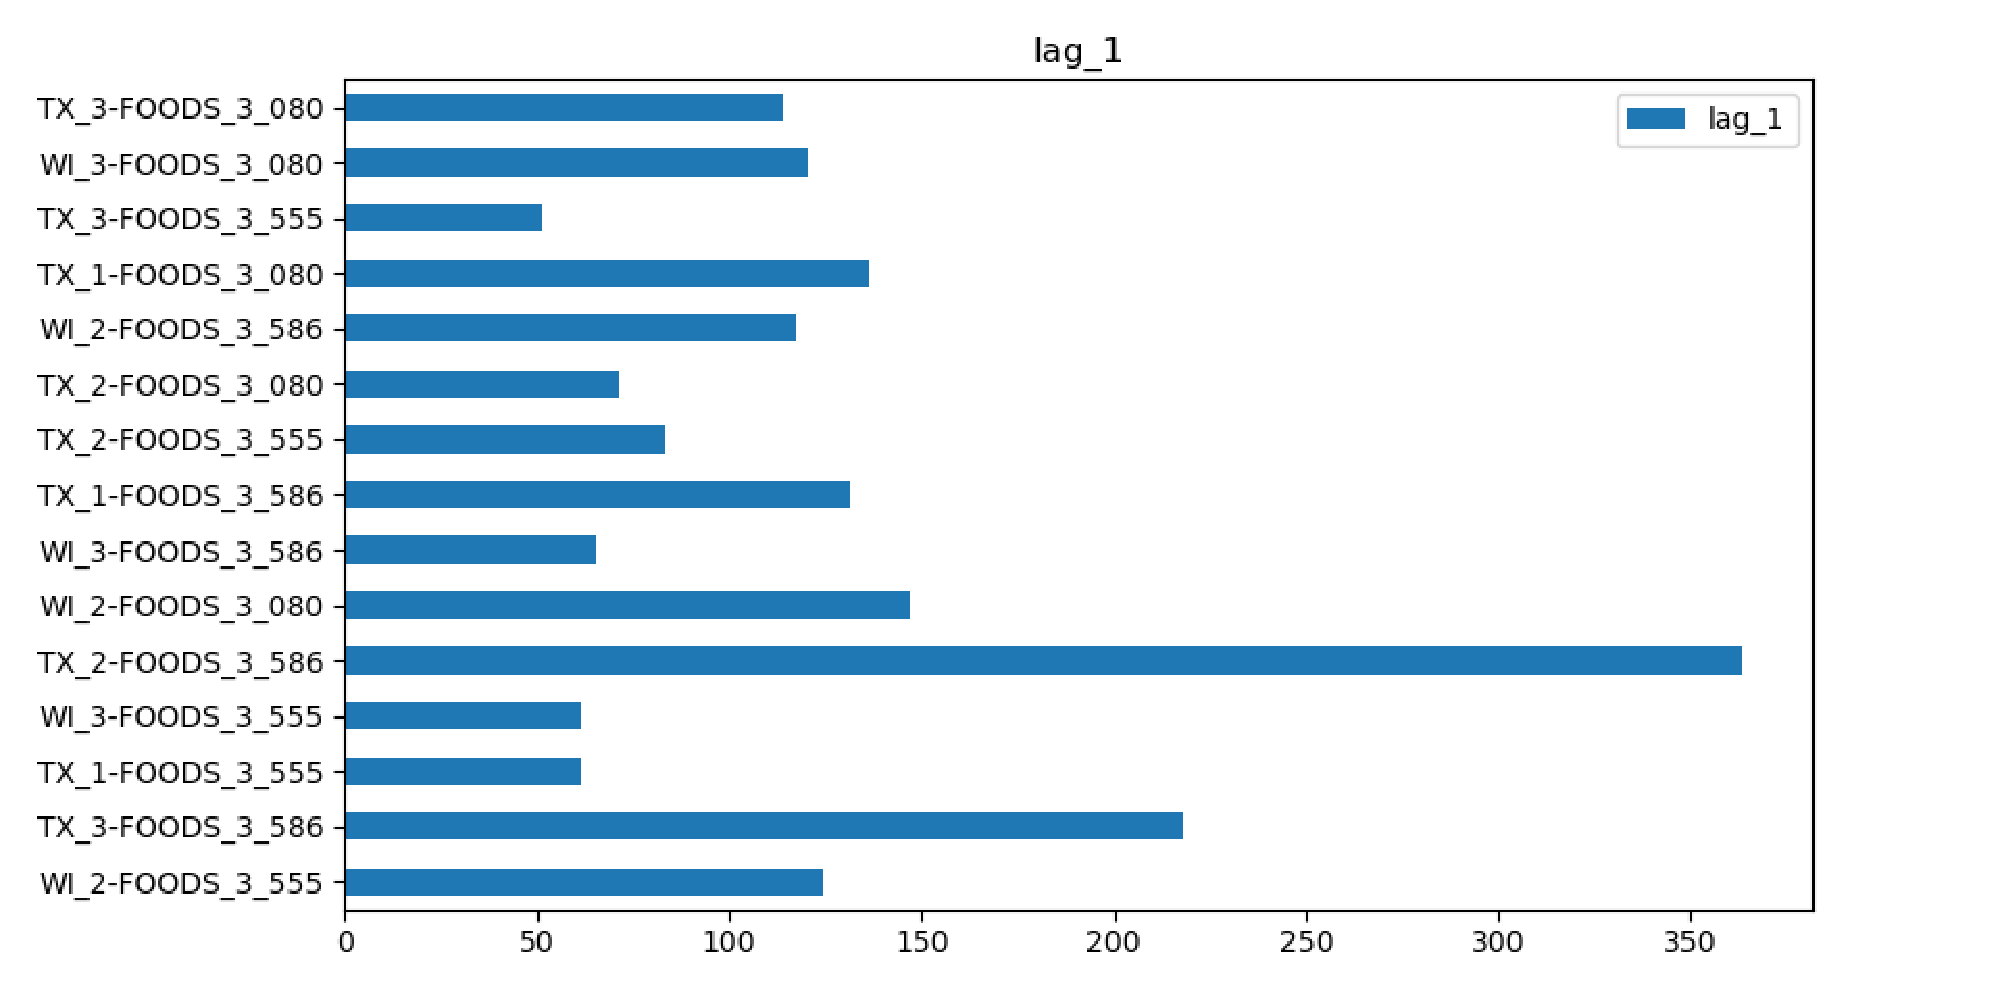
\includegraphics[width=0.8\linewidth]{sections/img/store_product_shap_2.eps}
        \caption{Store and product level SHAP values for one feature}
        \label{fig:store_product_sub2}
    \end{subfigure}%
    \vskip\baselineskip
    \begin{subfigure}{.5\textwidth}
        \centering
        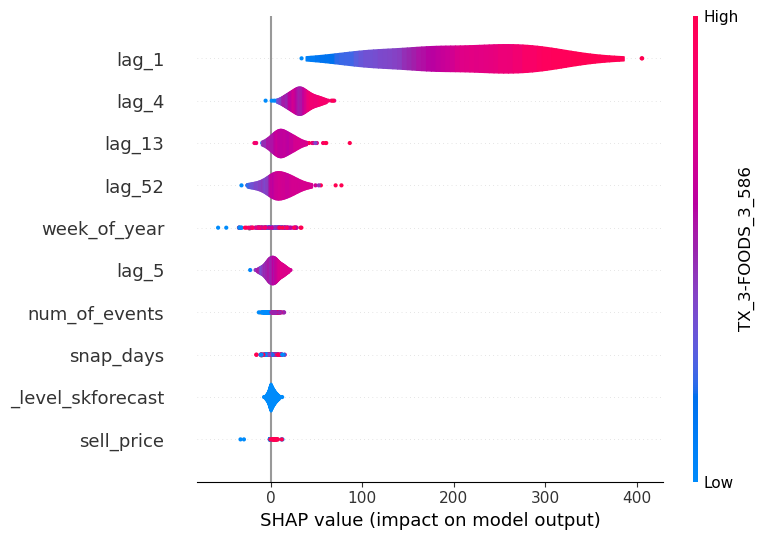
\includegraphics[width=\linewidth,]{sections/img/store_product_violin3}
        \caption{Store TX\_3 FOODS\_3\_586 product SHAP summary}
        \label{fig:store_prod_sub3}
    \end{subfigure}%
    \begin{subfigure}{.5\textwidth}
        \centering
        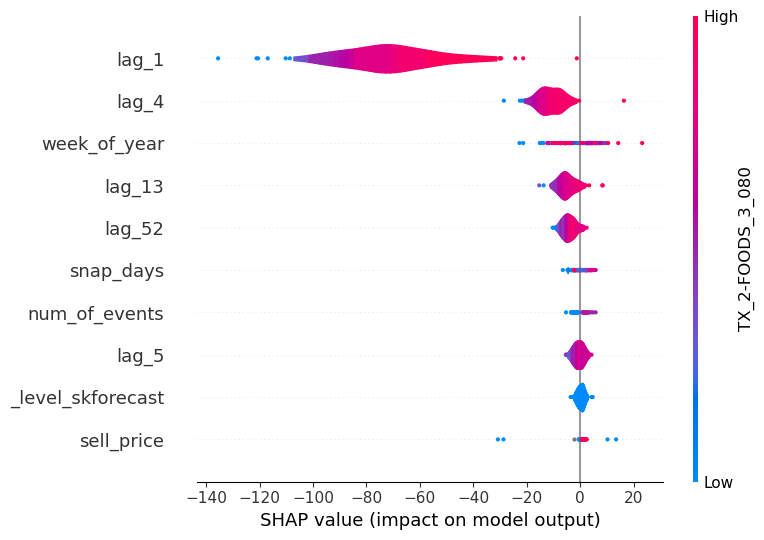
\includegraphics[width=\linewidth]{sections/img/store_productviolin2}
        \caption{Store TX\_2 FOODS\_3\_080 product SHAP summary}
        \label{fig:store_prod_violin_sub4e}
    \end{subfigure}
    \caption{Store and product level summary}\label{fig:store_product_summary}
\end{figure}



